% !TeX encoding = UTF-8
% !TeX spellcheck = pl_PL

\def\filename{rozdzial4}
\chapter{Metodyka badania}

\section{Model sieci neuronowej}

\subsubsection{Wstęp}
Badania przeprowadzono w środowisku Python z wykorzystaniem interaktywnego notatnika Jupyter Notebook.
Obliczenia wykonywano na komputerze wyposażonym w kartę graficzną NVIDIA GeForce RTX 5070 Ti, wspierającą akcelerację obliczeń w oparciu o technologię CUDA. 
Wykorzystanie GPU pozwoliło znacząco skrócić czas trenowania modeli konwolucyjnych oraz umożliwiło przeprowadzenie złożonych eksperymentów w rozsądnym czasie obliczeniowym.
	
Podczas konfiguracji i trenowania sieci neuronowych zastosowano zestaw bibliotek wspierających przetwarzanie danych, budowę modeli głębokiego uczenia oraz analizę wyników. 
Główne pakiety wykorzystane w badaniu to:
\begin{itemize}
	\item \textbf{pandas} - narzędzie do analizy danych tabelarycznych, umożliwiające ich wczytywanie, filtrowanie oraz łączenie metadanych z obrazami \cite{pandas},
	\item \textbf{numpy} - biblioteka numeryczna wykorzystywana do operacji na macierzach, wektorach oraz konwersji obrazów do formatów wejściowych modeli \cite{Harris_2020},
	\item \textbf{matplotlib} oraz \textbf{seaborn} – pakiety do wizualizacji danych, używane do generowania wykresów, prezentacji obrazów oraz analizy rozkładów klas \cite{matplotlib, seaborn},
	\item \textbf{tensorflow} oraz \textbf{keras} - pakiety głębokiego uczenia wykorzystywane do trenowania modeli konwolucyjnych oraz obsługi akceleracji GPU \cite{abadi2016tensorflowlargescalemachinelearning},
	\item \textbf{torch} oraz \textbf{torchvision} - biblioteki do budowy i trenowania sieci neuronowych, wykorzystywane do transformacji obrazów, przygotowania zbiorów danych oraz korzystania z gotowych architektur modeli \cite{1874254, paszke2019pytorchimperativestylehighperformance},
	\item \textbf{scikit-learn} - zestaw narzędzi do analizy predykcyjnej, umożliwiający podział danych na zbiory treningowe i testowe, obliczanie wag klas oraz ewaluację modeli \cite{pedregosa2018scikitlearnmachinelearningpython},
	\item \textbf{Pillow (PIL)} - biblioteka służąca do podstawowego przetwarzania obrazów, w tym ich wczytywania, skalowania i konwersji.
\end{itemize}

\subsection{Obróbka danych}
Zbiór PAD‑UFES‑20 pobrano lokalnie i załadowano z dysku, a następnie rozpakowano archiwa zdjęć.
W kolejnym kroku utworzono kolumnę path, która wskazywała pełną ścieżkę do konkretnego pliku graficznego. 
Umożliwiło to późniejsze elastyczne operowanie na obrazach.
	
\begin{lstlisting}[language=Python, caption=Funkcja do rozpakowywania archiwów ZIP]
def unzip(zip_path, extract_to):
	if not os.path.exists(zip_path):
		print(f"ZIP nie istnieje: {zip_path}")
		return
	os.makedirs(extract_to, exist_ok=True)
	with zipfile.ZipFile(zip_path, 'r') as zip_ref:
		zip_ref.extractall(extract_to)
\end{lstlisting}

Po rozpakowaniu zdjęć przypisano każdemu rekordowi dokładnej lokalizacji odpowiadającego mu obrazu na dysku.
Następnie przeprowadzono weryfikację integralności danych polegającą na próbie otwarcia każdego pliku graficznego.
Obrazy, które generowały wyjątek, zostały usunięte ze zbioru, co zapewniło poprawność danych wejściowych wykorzystywanych w dalszych etapach analizy.

\begin{lstlisting}[language=Python, caption=Funkcja do usuwania uszkodzonych obrazów]
def remove_corrupted(metadata, path_column="path"):
	good, bad = [], []
	for path in metadata[path_column]:
		try:
			if path is None or not os.path.exists(path):
				bad.append(path)
				continue
			img = Image.open(path)
			img.verify()
			good.append(path)
		except Exception:
			bad.append(path)
	return metadata[metadata[path_column].isin(good)].reset_index(drop=True)
\end{lstlisting}

Ze względu na silną nierównowagę klas zastosowano oversampling, czyli technikę polegającą na sztucznym zwiększeniu liczby przykładów klas rzadkich poprzez wielokrotne powielanie.
W efekcie liczebność kategorii SK, NEV, MEL oraz SCC została zwiększona do 300 przykładów.
Rozkład klas przed i po oversamplingu przedstawiono odpowiednio na wykresach \ref{fig:classes_bar}, \ref{fig:classes_pie} oraz \ref{fig:oversampling_classes}.

\begin{figure}[h!]
	\centering
	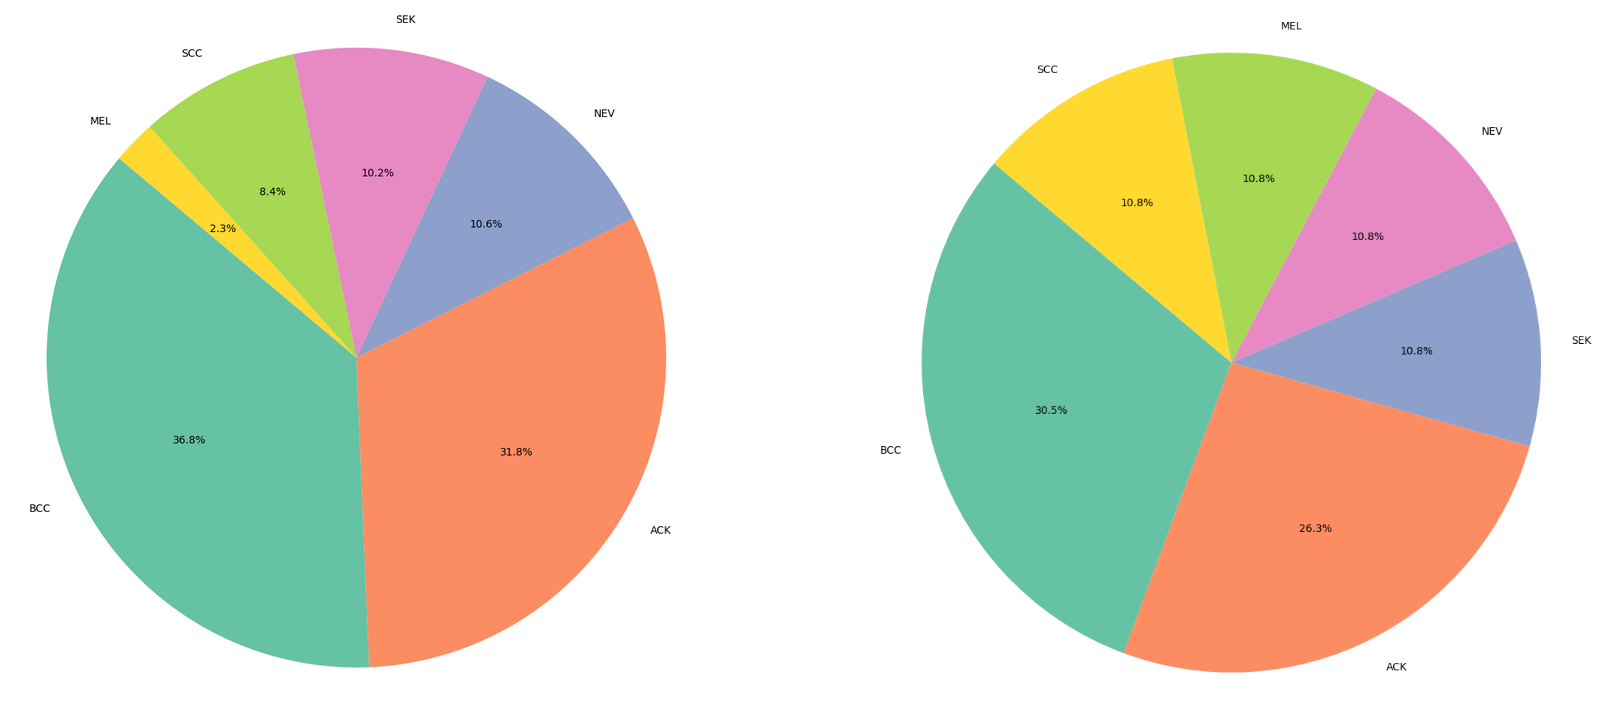
\includegraphics[width=0.9\linewidth]{oversampling_classes}
	\caption{Rozkład klas po oversamplingu}
	\source{Opracowanie własne}
	\label{fig:oversampling_classes}
\end{figure}

\subsubsection{Przygotowanie do trenowania}
Następnie wydzielono zbiór treningowy, testowy oraz walidacyjny w proporcjach:
\begin{itemize}
	\item dane treningowe - 1998 przykładów (72\% zbioru)
	\item dane walidacyjne - 222 przykładów (8\% zbioru)
	\item dane testowe - 555 przykładów (20\% zbioru)
\end{itemize}

W celu przygotowania danych do trenowania wykorzystano klasę ImageDataGenerator z biblioteki Keras, która umożliwia wykonywanie losowych transformacji obrazów podczas trenowania modelu.
Augmentacje danych wejściowych zwiększają różnorodność danych treningowych, co ogranicza ryzyko przeuczenia oraz lepiej odzwierciedla zmienność jakości zdjęć wykonywanych smartfonem.
Zastosowano następujące transformacje:
\begin{itemize}
	\item obrót obrazu o losowy kąt do 25 stopni
	\item przesunięcia poziome i pionowe do 15\% wymiaru obrazu
	\item przybliżenie do 25\%
	\item nachylenie obrazu do 10 stopni
	\item losowe odbicia poziome i pionowe
	\item zmiane jasności w zakresie 0.4-1.l6
	\item przesunięcie kanałów kolorystycznych do 40 jednostek
	\item uzupełnianie pikseli metodą nearest
\end{itemize}

Agresywne transformacje pozwalają modelowi uczyć się bardziej odpornych reprezentacji, szczególnie istotnych w przypadku zdjęć wykonywanych w warunkach domowych, przy zmiennym oświetleniu i różnej jakości aparatów.
Dla zbiorów walidacyjnych i testowych zastosowano generatory bez augmentacji, aby zapewnić obiektywną i powtarzalną ocenę jakości modelu.

\begin{lstlisting}[language=Python, caption=Definicja ImageDataGeneratora dla klasy treningowej]
train_datagen = ImageDataGenerator(
	preprocessing_function=preprocess_input,
	rotation_range=10,
	zoom_range=0.1,
	horizontal_flip=True,
	fill_mode='nearest'
)
\end{lstlisting}

Następnie utworzono generatory wczytujące obrazy z dysku, skalujące je do rozmiaru 299 na 299 pikseli, kodujące etykiety oraz stosujące zdefiniowane transformacje.

W celu porównania skuteczności rożnych architektur konwolucyjnych sieci neuronowych zdefiniowano słownik modeli dostępnych w ramach biblioteki Keras.
Modele różnią się pod względem liczby parametrów, głębokości architektury oraz przeznaczenia.
Część z wybranych sieci zostało zaprojektowanych specjalnie z myślą o urządzeniach mobilnych, co jest istotne w kontekście implementacji systemu wykonującego inferencję na smartfonie.

\begin{lstlisting}[language=Python, caption=Słownik sieci neuronowych]
MODELS = {
	"MobileNetV2": tf.keras.applications.MobileNetV2,
	"MobileNetV3Large": tf.keras.applications.MobileNetV3Large,
	"ResNet50": tf.keras.applications.ResNet50,
	"EfficientNetB0": tf.keras.applications.EfficientNetB0,
	"DenseNet121": tf.keras.applications.DenseNet121,
	"ResNet101": tf.keras.applications.ResNet101,
	"ConvNeXtTiny": tf.keras.applications.ConvNeXtTiny,
}
\end{lstlisting}

\subsubsection{Przygotowanie do trenowania}
Aby umożliwić elastyczne trenowanie wielu modeli, stworzono wysokopoziomowy moduł TransferLearningTuner, który kompleksowo obsługuje cały proces trenowania z wykorzystaniem techniki transfer learning.
Konstruktor klasy przyjmuje między innymi nazwę modelu bazowego zdefiniowaną w słowniku, liczbę klas, generatory danych oraz parametry trenowania.

TransferLearningTuner w pierwszym kroku tworzy architekturę wczytując model bazowy i zamrażając jego wagi, co zapobiega degradacji wcześniej wyuczonych reprezentacji.
W kolejnym kroku dodano warstwy klasyfikacyjne, które redukują wymiar cech, stabilizują trenowanie oraz zapobiegają przeuczeniu.

Pierwszy etap trenowania polega na uczeniu wyłącznie warstw klasyfikacyjnych przy zamrożonych wagach modelu bazowego.
Domyślnie trenowanie w tym etapie składa się z pięciu epok.
Do trenowania wykorzystano optymalizator Adam oraz funkcję straty CategoricalCrossentropy, która redukuje wpływ klas dominujących na predykcje modelu.
Zdefiniowano również kilka funkcji wywoływanych po każdej epoce lub po zakończeniu procesu, polegających na zapisie najlepszych wag modelu, zatrzymanie trenowania po 3 epokach bez poprawy, redukcji learning rate przy stagnacji oraz minitorowanie różnic między domeną dermoskopową a zdjęć telefonicznych.

Drugi etap trenowania odmraża większość warstw modelu bazowego z wyjątkiem warstw BatchNormalization, które przechowują statystyki domenowe i ich trenowanie mogłoby destabilizować proces.
Odmrożenie warstw pozwala dostosować głębsze reprezentacje do specyfiki danych dermatologicznych.

Po zakończeniu trenowania wykonywana jest ewaluacja na zbiorze testowym a następnie generowana jest macierz pomyłek, wynik F1 dla każdej klasy oraz wykresy strat i dokładności.
Następnie wytrenowany model jest konwertowany do formatu TensorFlow Lite, umożliwiając wykorzystanie go do bezpośredniej inferencji na urządzeniu mobilnym.
Cały pipeline uruchamiany jest metodą run, która wykonuje oba etapy trenowania oraz pełną ewaluację.

\section{Aplikacja mobilna}
W ramach stworzenia prototypu systemu zaprojektowano aplikację mobilną wykorzystującą wytrenowany model klasyfikacji zmian skórnych.
Aplikację zaimplementowano na platformę Android z użyciem języka Kotlin oraz biblioteki Jetpack Compose, która umożliwia deklaratywne tworzenie interfejsu użytkownika.
Model sieci neuronowej został umieszczony w zasobach aplikacji i obsłużony za pomocą biblioteki TensorFlow Lite.

\begin{figure}[h!]
	\centering
	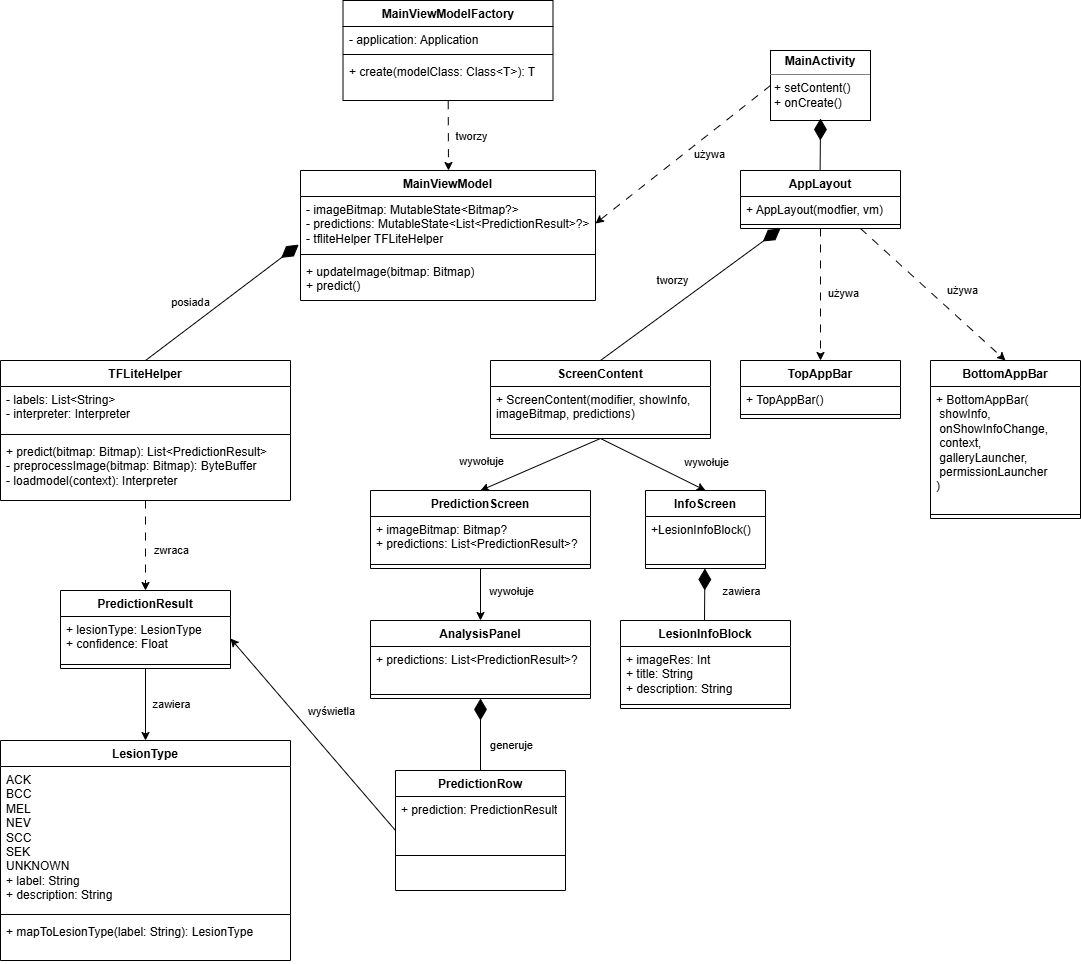
\includegraphics[width=1\linewidth]{diagram_klas}
	\caption{Diagram klas przedstawiający działanie aplikacji}
	\source{Opracowanie własne}
	\label{fig:diagram_klas}
\end{figure}

Diagram \ref{fig:diagram_klas} przedstawia pełną architekturę aplikacji, w której warstwa interfejsu użytkownika jest oddzielona od logiki przetwarzania obrazu oraz inferencji modelu.
Głównym punktem wejścia aplikacji jest klasa \texttt{MainActivity}, odpowiedzialna za inicjalizację środowiska Jetpack Compose.
Klasa ta korzysta z \texttt{MainViewModel}, który zarządza stanem aplikacji.

Po stronie interfejsu użytkownika kluczową rolę pełni komponent \texttt{AppLayout}, tworzony w ramach \texttt{MainActivity}.
Odpowiada on za ogólny układ aplikacji, w tym wyświetlanie górnego i dolnego paska nawigacyjnego (\texttt{TopAppBar} oraz \texttt{BottomAppBar}) oraz za inicjalizację głównego obszaru roboczego.
\texttt{AppLayout} tworzy komponent \texttt{ScreenContent}, który decyduje o tym, jaki ekran zostanie wyświetlony - ekran klasyfikacji (\texttt{PredictionScreen}) lub ekran informacyjny (\texttt{InfoScreen}), zależnie od stanu \texttt{showInfo} przechowywanego w \texttt{MainViewModel}.

Ekran \texttt{PredictionScreen} odpowiada za wyświetlanie instrukcji oraz wyników klasyfikacji.
Jeżeli użytkownik nie wykonał jeszcze zdjęcia, \texttt{PredictionScreen} prezentuje komunikat z instrukcją dotyczącą wykonania fotografii zmiany skórnej.
Po wykonaniu zdjęcia i przetworzeniu go przez model wywoływany jest komponent \texttt{AnalysisPanel}, który generuje dynamiczną listę elementów \texttt{PredictionRow}.
Każdy z nich reprezentuje pojedynczy wynik inferencji, zawierający typ zmiany skórnej oraz poziom pewności klasyfikacji.
Ekran \texttt{InfoScreen} pełni funkcję informacyjną.
Zawiera zestaw bloków \texttt{LesionInfoBlock}, prezentujących opisy wszystkich typów zmian skórnych zdefiniowanych w enumeracji \texttt{LesionType} oraz informacje na temat projektu.

Logika przetwarzania obrazu oraz komunikacja z modelem TensorFlow Lite została umieszczona w dedykowanej klasie \texttt{TFLiteHelper}.
Klasa ta jest tworzona i przechowywana wewnątrz \texttt{MainViewModel}, co zapewnia jej spójny cykl życia.
\texttt{TFLiteHelper} odpowiada za przygotowanie danych wejściowych, w tym skalowanie obrazu, konwersję do formatu \texttt{ByteBuffer} oraz zastosowanie preprocessingu zgodnego z architekturą modelu.
Wynik inferencji stanowi wektor prawdopodobieństw, który jest mapowany na typy zmian skórnych zdefiniowane w \texttt{LesionType}.
Każdy wynik jest reprezentowany jako obiekt \texttt{PredictionResult}.

Przepływ danych w aplikacji odzwierciedla naturalny scenariusz użytkownika.
Proces rozpoczyna się od wykonania zdjęcia lub wyboru obrazu z galerii.
\texttt{MainViewModel} aktualizuje stan \texttt{imageBitmap}, a następnie wywołuje metodę \texttt{predict()} w klasie \texttt{TFLiteHelper}.
Otrzymane wyniki są przekazywane do warstwy prezentacji i wyświetlane w komponencie \texttt{PredictionScreen} w postaci listy obiektów \texttt{PredictionResult}.
Użytkownik może również przełączyć się do zakładki Info, w której komponent \texttt{InfoScreen} prezentuje szczegółowe opisy wszystkich typów zmian skórnych.
Pełen przepływ użytkownika wraz z prezentacją interfejsu przedstawiono na diagramach \ref{fig:diagram_app1} oraz \ref{fig:diagram_app2}.


\begin{figure}[h!]
	\centering
	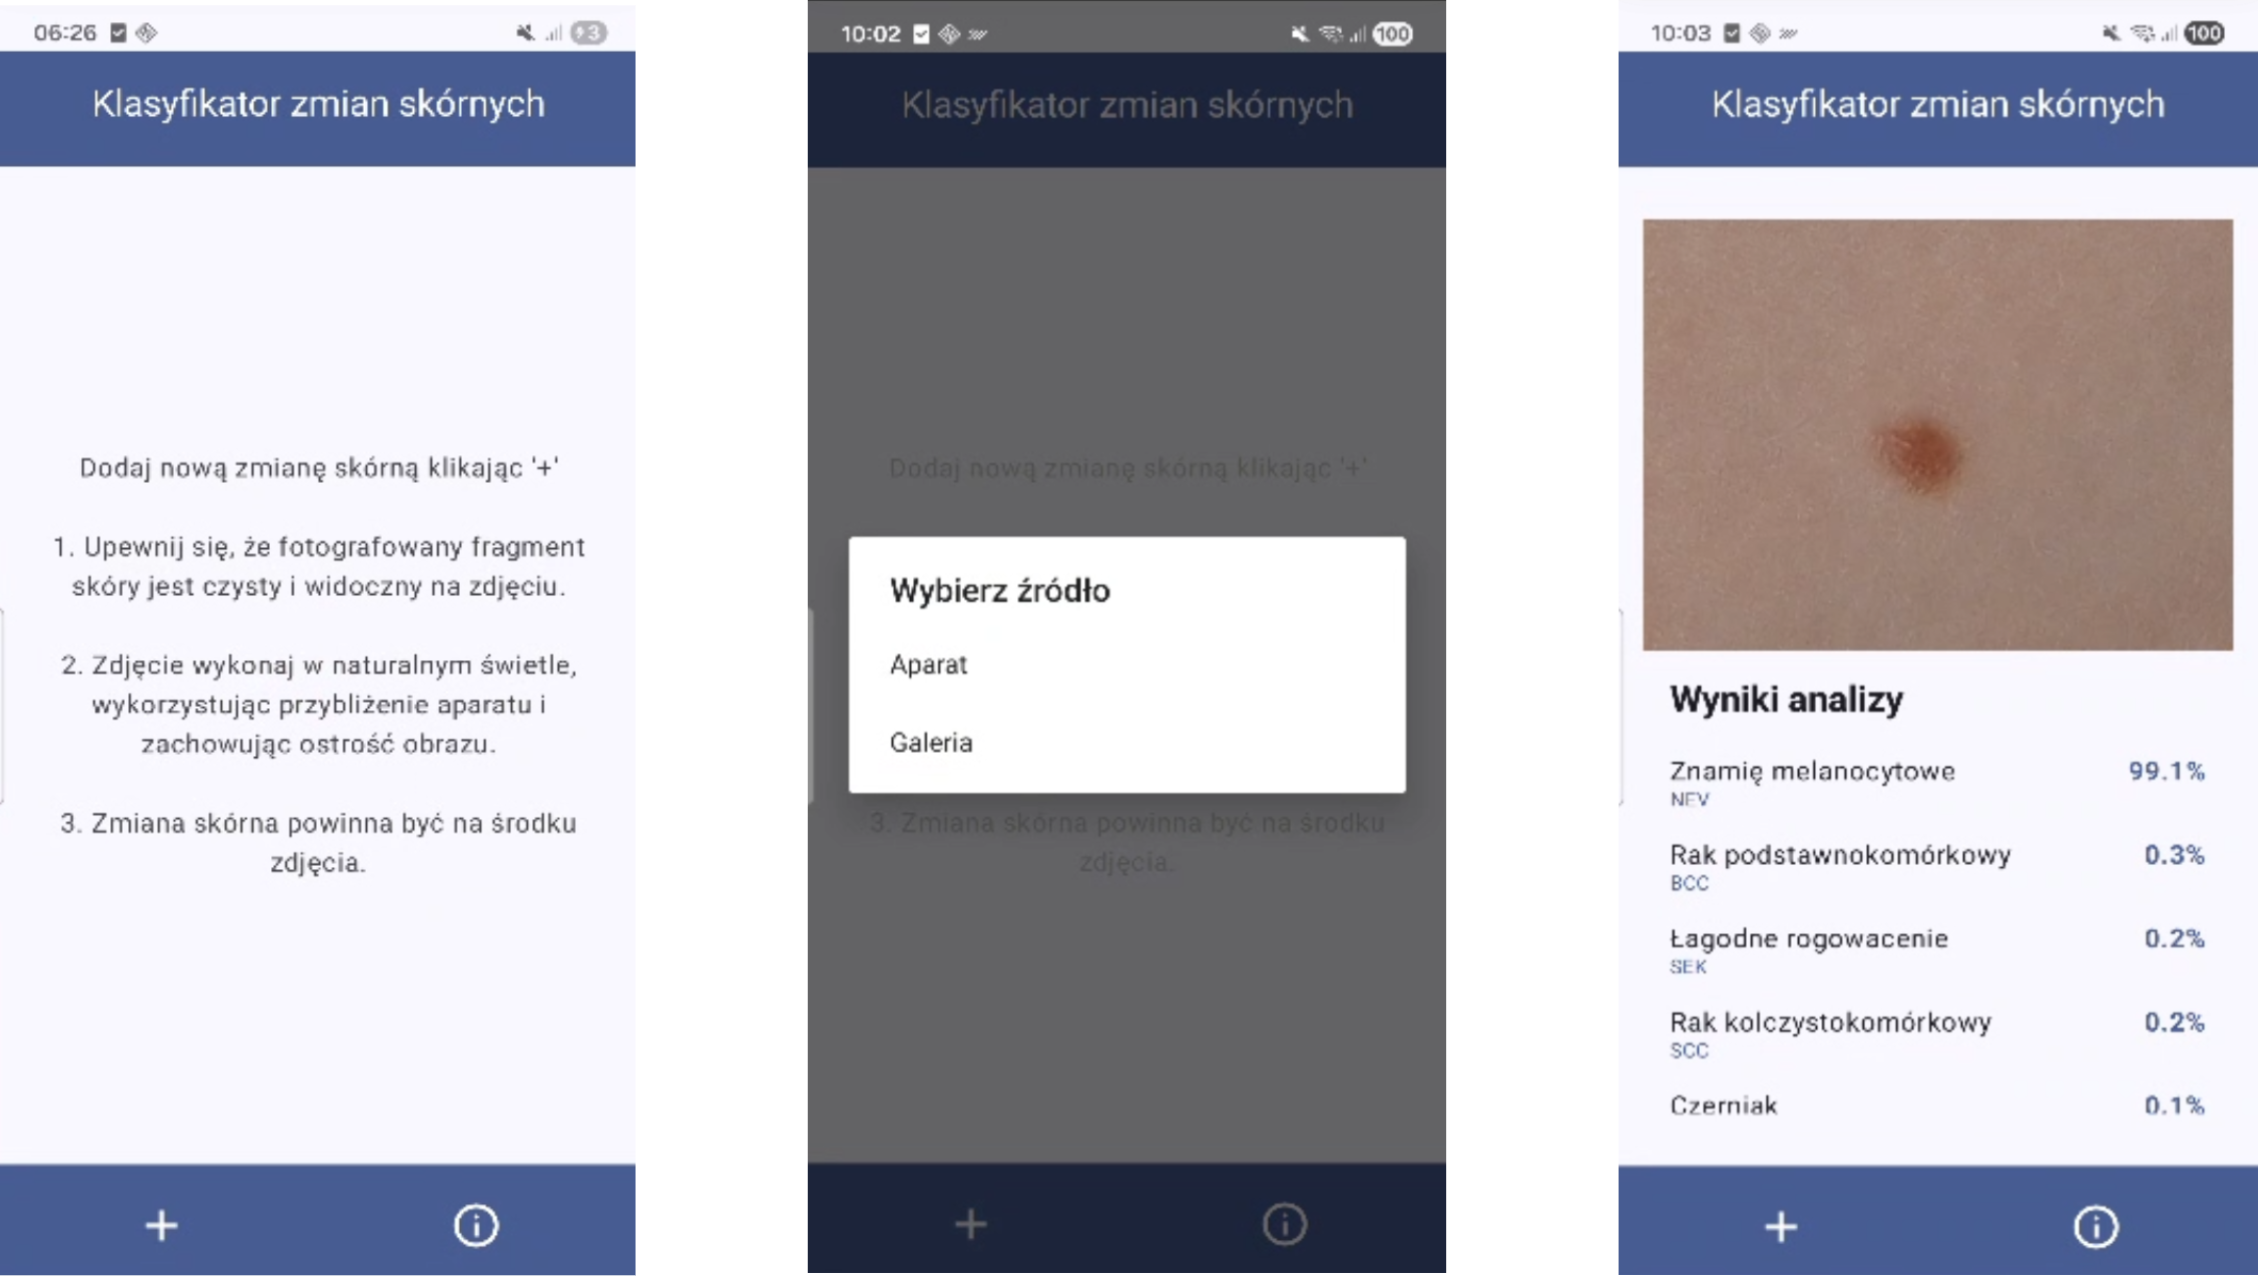
\includegraphics[width=0.9\linewidth]{diagram_app1}
	\caption{Diagram klas przedstawiający przepływ użytkownika przez proces klasyfikacji zmiany skórnej}
	\source{Opracowanie własne}
	\label{fig:diagram_app1}
\end{figure}


\begin{figure}[h!]
	\centering
	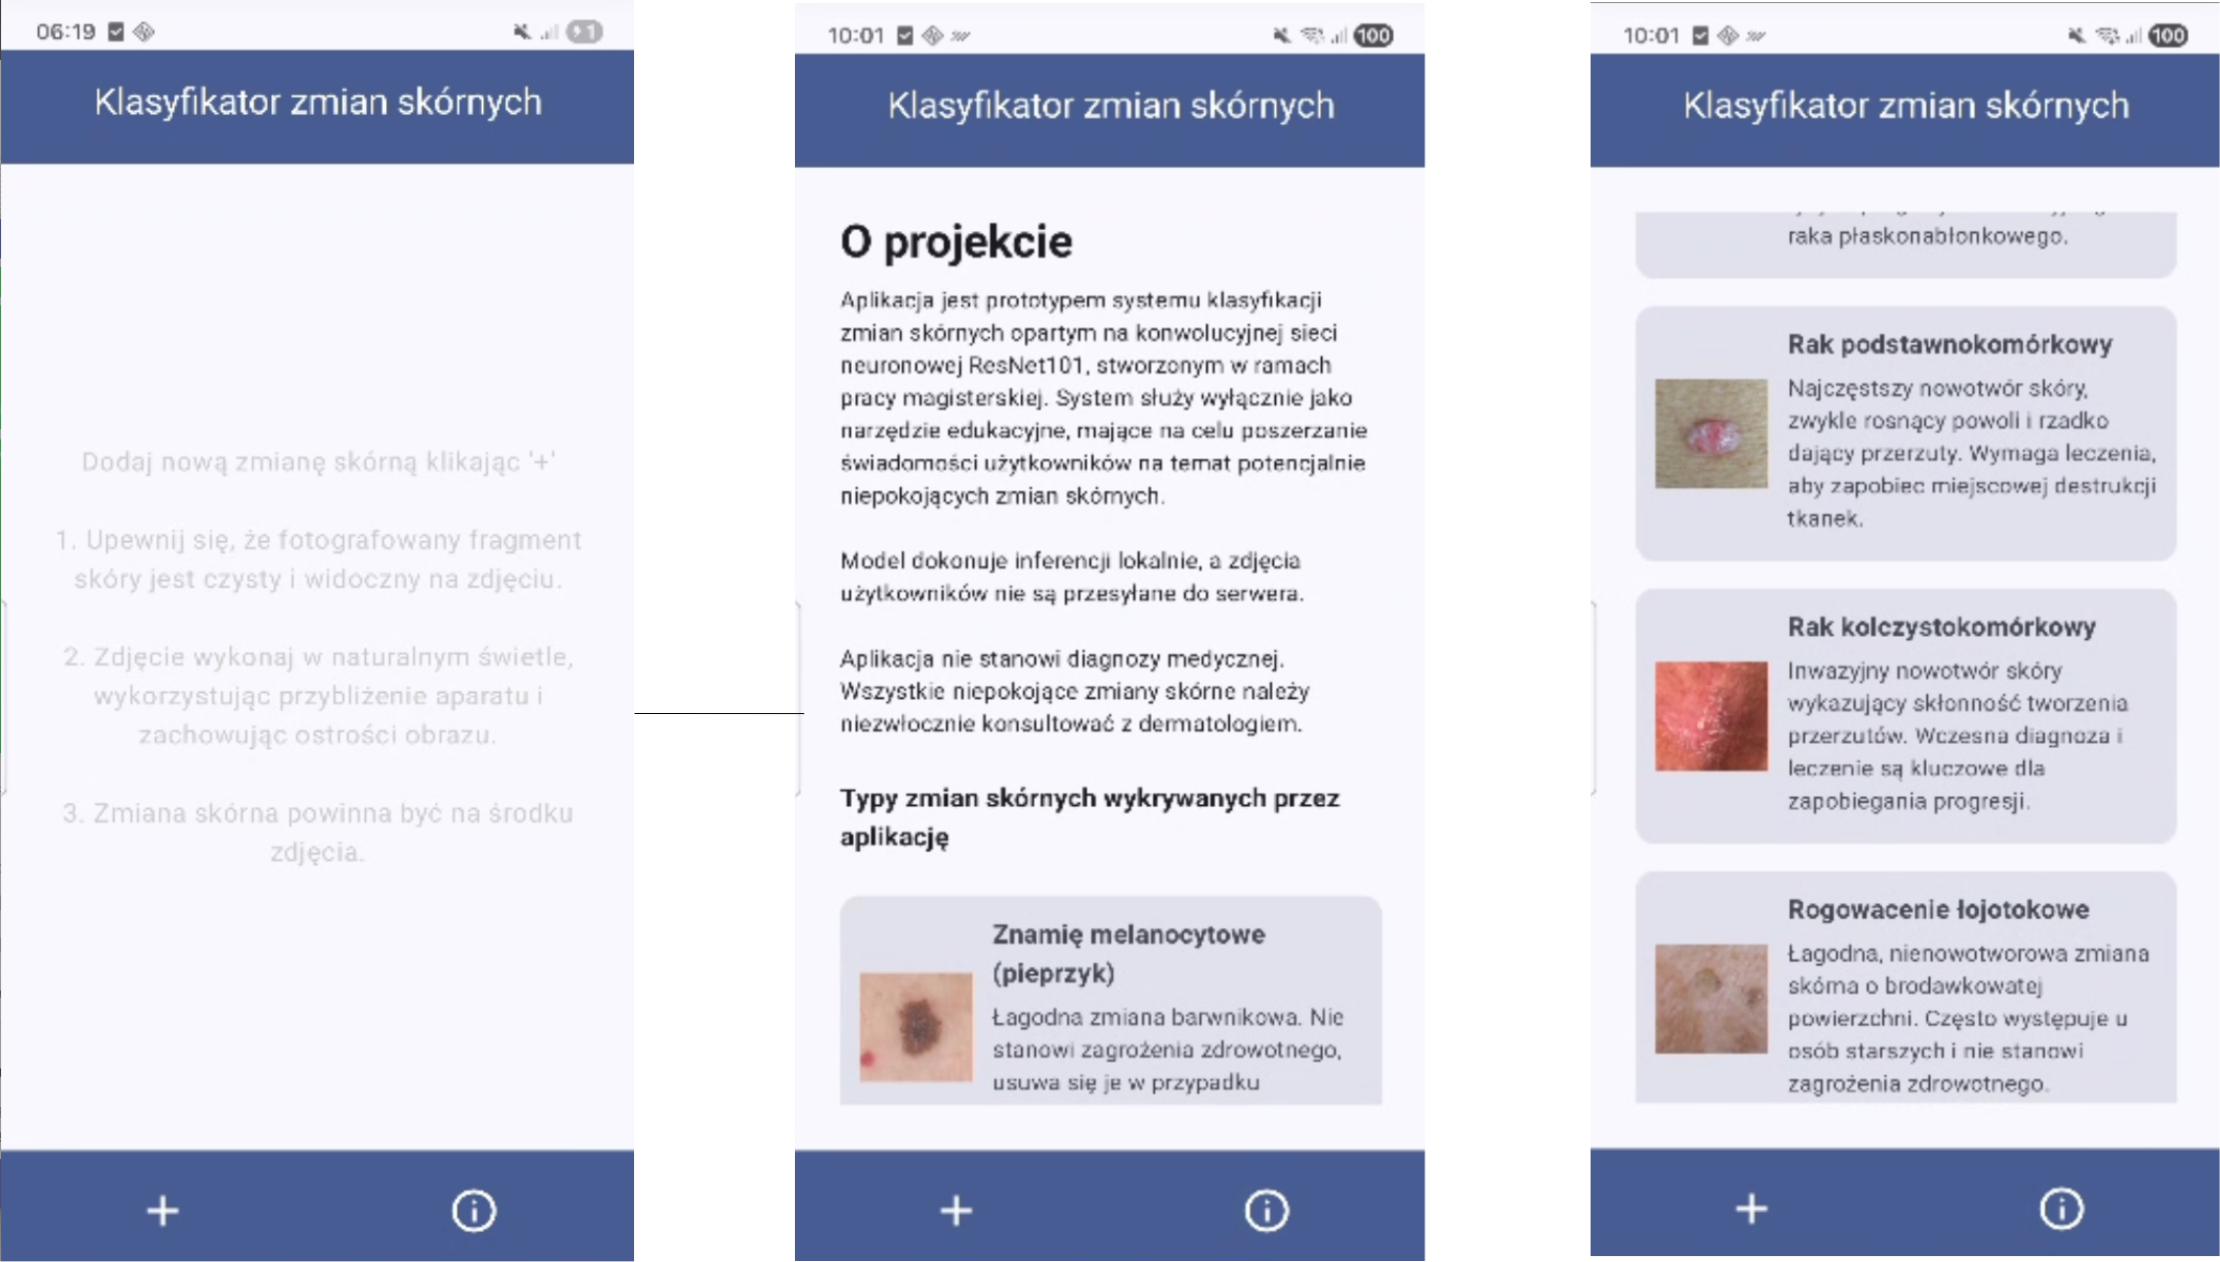
\includegraphics[width=0.9\linewidth]{diagram_app2}
	\caption{Diagram klas przedstawiający InfoScreen}
	\source{Opracowanie własne}
	\label{fig:diagram_app2}
\end{figure}


\section{Wyniki}


\section{Podsumowanie}